\documentclass[10pt]{article}
\usepackage{multirow}
\usepackage{bigdelim}
\usepackage{color}

%Math
\usepackage{amsmath}
\usepackage{amsfonts}
\usepackage{amssymb}
\usepackage{amsthm}
\usepackage{ulem}
\usepackage{stmaryrd} %f\UTF{00FC}r Blitz!

%PageStyle
\usepackage[ngerman]{babel} % deutsche Silbentrennung
\usepackage[utf8]{inputenc} 
\usepackage{fancyhdr, graphicx}
\usepackage[scaled=0.92]{helvet}
\usepackage{enumitem}
\usepackage{parskip}
\usepackage[a4paper,top=2cm]{geometry}
\setlength{\textwidth}{17cm}
\setlength{\oddsidemargin}{-0.5cm}


% Shortcommands
\newcommand{\Bold}[1]{\textbf{#1}} %Boldface
\newcommand{\Kursiv}[1]{\textit{#1}} %Italic
\newcommand{\T}[1]{\text{#1}} %Textmode
\newcommand{\Nicht}[1]{\T{\sout{$ #1 $}}} %Streicht Shit durch

%Arrows
\newcommand{\lra}{\leftrightarrow} 
\newcommand{\ra}{\rightarrow}
\newcommand{\la}{\leftarrow}
\newcommand{\lral}{\longleftrightarrow}
\newcommand{\ral}{\longrightarrow}
\newcommand{\lal}{\longleftarrow}
\newcommand{\Lra}{\Leftrightarrow}
\newcommand{\Ra}{\Rightarrow}
\newcommand{\La}{\Leftarrow}
\newcommand{\Lral}{\Longleftrightarrow}
\newcommand{\Ral}{\Longrightarrow}
\newcommand{\Lal}{\Longleftarrow}

% Code listenings
\usepackage{color}
\usepackage{xcolor}
\usepackage{listings}
\usepackage{caption}
\DeclareCaptionFont{white}{\color{white}}
\DeclareCaptionFormat{listing}{\colorbox{gray}{\parbox{\textwidth}{#1#2#3}}}
\captionsetup[lstlisting]{format=listing,labelfont=white,textfont=white}
\lstdefinestyle{JavaStyle}{
 language=Java,
 basicstyle=\footnotesize\ttfamily, % Standardschrift
 numbers=left,               % Ort der Zeilennummern
 numberstyle=\tiny,          % Stil der Zeilennummern
 stepnumber=5,              % Abstand zwischen den Zeilennummern
 numbersep=5pt,              % Abstand der Nummern zum Text
 tabsize=2,                  % Groesse von Tabs
 extendedchars=true,         %
 breaklines=true,            % Zeilen werden Umgebrochen
 frame=b,         
 %commentstyle=\itshape\color{LightLime}, Was isch das? O_o
 %keywordstyle=\bfseries\color{DarkPurple}, und das O_o
 basicstyle=\footnotesize\ttfamily,
 stringstyle=\color[RGB]{42,0,255}\ttfamily, % Farbe der String
 keywordstyle=\color[RGB]{127,0,85}\ttfamily, % Farbe der Keywords
 commentstyle=\color[RGB]{63,127,95}\ttfamily, % Farbe des Kommentars
 showspaces=false,           % Leerzeichen anzeigen ?
 showtabs=false,             % Tabs anzeigen ?
 xleftmargin=17pt,
 framexleftmargin=17pt,
 framexrightmargin=5pt,
 framexbottommargin=4pt,
 showstringspaces=false      % Leerzeichen in Strings anzeigen ?        
}

%Config
\renewcommand{\headrulewidth}{0pt}
\setlength{\headheight}{15.2pt}

%Metadata
\fancyfoot[C]{If you use this documentation for a exam, you should offer a beer to the authors!}
\title{
	\vspace{5cm}
	Kryptographie
}
\author{Jan Fässler}
\date{3. Semester (HS 2012)}


% hier beginnt das Dokument
\begin{document}

% Titelbild
\maketitle
\thispagestyle{fancy}

\newpage

% Inhaltsverzeichnis
\pagenumbering{Roman}
\tableofcontents	  	


\newpage
\setcounter{page}{1}
\pagenumbering{arabic}

% Inhalt Start

\section{Klassische Kryptologie}
\subsection{Repetitionen}
\begin{description}
	\item[Alphabet] endliche Mengen von Zeichen
	\item[Beispiel] \hfill \\
		$\Lambda := \{A,B,C, ..., Z\}$, $|\Lambda|=26$ \\
		$\Sigma := \{0,1\}$, $|\Sigma|=2$
\end{description}
Sprache über $\Lambda$ : $L \subset \Lambda$*

\subsection{Klassifizierungen}
\begin{tabular}{l | l}
	\textbf{Substitution Cipher} & \textbf{Transposition Cipher} \\
	\hline \\
	Einheiten werden \textbf{ersetzt}. & Einheiten werden \textbf{vertauscht}. \\
	& \begin{tabular}{c c c c c c}
		3 & 1 & 5 & 6 & 2 & 4 \\
		K & O & M & M & E & H \\
		E & U & T & E & A & B \\
		E & N & D & Z & U & M \\
		Z & O & O & A & B & C \\
	\end{tabular} \\
	& ABC = padding  \\
	& $\ra$ OUNOEAUBK... 
\end{tabular} \\ \\
\\
\begin{tabular}{l | l}
	\textbf{mono-alphabetische Cipher} & \textbf{poly-alphabetische Cipher} \\
	\hline \\
	$E: A\ra B$ & $E: A \ra P(B)$ \\
	$x \ra E(x)$ & $x \ra E(x)$ \\
	Buchstaben & Gruppen von Buchstaben \\
\end{tabular}

\subsection{Homophone Verschlüsselung}
\begin{description}
	\item[Gegeben] $\sum := \{0,1\}$, $B:=\{a,b,c\}$
\end{description}
Informationen über die Sprache des Klartextes: \\
Häufigkeit von $0=\frac{1}{3}$ \\
Häufigkeit von $1=\frac{2}{3}$
\begin{align}
	E: & \sum \ra P_{(B)} \\
	& 0 \ra \{b\} \\
	& 1 \ra \{a,c\}
\end{align}
Beispiel: \\
10110110011 \\
abccbacbbaa

\subsection{Kaski - Text}
\begin{description}
	\item[Klartext] TO BE OR NOT TO BE
	\item[Schlüssel] NOW
\end{description}

\begin{tabular}{l l l | l l l | l l l | l l l | l }
	T & O & B & E & O & R & N & O & T & T & O & B & E \\ 
	N & O & W & N & O & W & N & O & W & N & O & W & N \\
	G & C & X & R & C & N & A & C & P & G & C & X & R \\
	$-$ & $-$ & $-$ & $-$ & & & & & & $-$ & $-$ & $-$ & $-$ \\
\end{tabular}

\subsection{Polyfair-Cipher}
tbd.

\subsection{Koinzidenzindex}
\begin{description}
	\item[1) Gegeben] \hfill \\
		Alphabet $\Lambda := \{A,B,C, ..., Z\}$ \\
		Sprache: Englisch \\ 
		$\ra$ Buchstabenhäufigkeit: 
		\begin{tabular}{c c c c}
			$p_A$ & $p_B$ & ... & $p_Z$ \\
			" & " & & " \\
			$p_1$ & $p_2$ & ... & $p_3$ \\
		\end{tabular} \\
		mit $0\leq p_i \leq 1$ und $\sum_{i=1}^{26} p_i=1$
	\item[IC:] Grösse, die von der Sprache abhängt, aber invariant ist gegenüber Cäsar-Verschiebungen.
	\item[Frage:] Was bedeutet: $IC_L := \sum_{i=1}^{26} p_i^2$ ?
	\item[Bemerkung:] \hfill \\
		Jede Sprache hat ihren eigenen Konzidenzindex \\
		$IC_{German}=0.0766$ \\
		$IC_{Arabic}=0.0759$ \\
		$IC_{flat}=0.0385$ (Alle Buchstaben haben die gleiche häufigkeit: $p_1=p_2=...=p_{26}=\frac{1}{26}$)\\
		\textbf{Je unregelmässiger die buchstabenhäufigkeit, umso grösser der Index.}
	\item[2) Gegegen:] \hfill \\
		Sei F eine buchstabenfolge der Länge n \\
		Bsp: F= "{}AXCAABCXA"
	\item[Frage:] Wie gross ist die Wahrscheinlichkeit zwei gleiche Buchstaben aus F herauszugreifen?
	\item[Definition] $IC_F=\frac{\sum_{i=1}^{26} \binom{n_i}{2}}{\binom{n}{2}}$
	\item[Bsp:] \hfill \\
		Alphabet $\Sigma := \{0,1\}$ \\
		F = 00110111101 \\
		\begin{tabular}{l l}
			\begin{tabular}{l}
				$n_0=4$ \\
				$n_1=7$ \\
				\hline
				$n=11$ \\
			\end{tabular} & $\}$ $IC_F=\frac{4*3+7*6}{11*10}=0.49$ \\
		\end{tabular}
	\item[Annahme] $IC_F  \xrightarrow[F \ra \infty ]{}$ $IC_L$ ($i*A$ ist das falsch)
	\item[Bemerkung] \hfill \\
		Permutation der buchstaben \\
		F $\ra$ Perm(F) \\
		F = "{}AXCA ...." $\ra$ Perm(F) = "{}CBYC..." \\
		$IC_F=IC_{Perm(F)}$
\end{description}
\subsection{Vigenères Chipres}
\subsubsection{Berechnung der Schlüssellänge}
\begin{description}
	\item[Gegeben] \hfill \\
		C Vigenère-Chiffrat der Länge n \\
		Die Schlüssellänge sei p (unbekannt) \\ \\
		p = Spalten \\
		\begin{tabular}{ c c c c c l}
			$C_1$ & $C_2$ & $C_3$ & ... & $C_p$ & $\rdelim\}{4}{1cm}[n/p]$\\
			$C_{p1}$ & $C_{p2}$ & $C_2$ & ... & $C_{2p}$  \\
			.. & .. & .. & .. & ..  \\
			$C_{n-2}$ & $C_{n-1}$ & $C_n$ & $-$ & $-$ \\
		\end{tabular}
		
		\begin{description}
			\item[$\alpha :=$] Anzahl Buchstabenpaare aus gleicher Spalte \\
				$\alpha = \frac{n(\frac{n}{p}-1)}{2} = \frac{n(n-p)}{2p}$
			\item[$\beta :=$] Anzahl Buchstabenpaare aus verschiedenen Spalte \\
				$\beta = \frac{n(n-\frac{n}{p})}{2} = \frac{n^2(p-1)}{2p}$
			\item[$\gamma :=$] Anzahl gleicher Buchstabenpaare aus C \\
				$IC_c=\frac{\gamma}{\binom{n}{2}}$ \\
				$\gamma = \alpha * IC_L + \beta * IC_{flat}$
		\end{description}
	\item[Beispiel] \hfill \\
		$p=\frac{n(IC_L-IC_{flat})}{IC_C(n-1)+IC_L-n*IC_{flat}}$
\end{description}

\subsubsection{Kryptoanalysis}
\begin{description}
	\item[1)] Schlüssellänge p\\
		p=1,2,3,...
		\begin{itemize}
			\item Einleitung des Cipher-Tests in p Abschnitte
			\item Berechnung des IC des Abschnitts
			\item Wähle p mit $IC\sim IC_2$ (oder hoch)
		\end{itemize}
	\item[2)] Sei s,t zwei  Strings über dem Alphabet A. \\
		$s=s_1,s_2,s_3, .... s_k$ \\
		$t=t_1,t_2,t_3, ..., t_l$ \\
		Wieder zählen wir $n_1(s) :=$ A in s, $n_3(t)=$ C in t
	\item[Def.] $MIC(s,t):=\frac{\sum_{i=1}{26}n_i(s)*n_i(t)}{k*l}$ \\
	\item[Bsp.] \hfill \\
		s="{}AABCCA" \\
		t="ABCABCABC" \\
		\\
		$n_1(s)=3$, $n_1(t)=3$ \\
		$n_2(s)=1$, $n_2(t)=3$ \\
		$n_3(s)=2$, $n_3(t)=3$ \\ \\
		$\ra$ $MIC(s,t)=\frac{1}{6*9}[3*3+1*3+2*3]$
	\item[Idee:] s,t zwei cipher-Text mit Cäsar Cerschlüsselung \\
		Wenn beide mit dem gleichen Schlüssel verschlüsselt werden \\
		$\ra$ $MIC(s,t)\rightsquigarrow IC_L$ \\
		Sonst: $MIC(s,t)\rightsquigarrow IC_{flat}$
	\item[3.)] \textbf{Anwendung auf Cipher Text} \\
		Schlüssellänge p sei 5 \\
		$c_1,c_2, ...,c_5$ Abschnitte des Cipher Text \\
		$MIC(c_i,c_j+k)$ \\ \\
		\textbf{Tabelle}:  \\
		\begin{tabular}{l | l l l l l}
			$k_{ij}\backslash k$ & 0 & 1 & 2 & 3 & ... \\
			\hline 
			(1,2) \\
			(1,3) \\
			(1,4) \\
			(1,5) \\
			(2,3) & & & x \\
			(2,4) \\
			(2,5) \\
			(3,4) \\
			(3,5) \\
			(4,5) \\
		\end{tabular} $\ra$ $MIC(c_2,c_3+k)$
	\item[Bsp] \hfill \\
		\begin{tabular}{l l}
			$c_1$: & AXBM...\\
			$c_3$: & ABXHE... \\
			\hline
			$c_3+2$: & CDZJG \\
		\end{tabular}
	\item[4.)] Wir suchen Einträge in der Tabelle, die hoch sind ($> 0.06$) \\
		zb: $MIC(c_2,c_3{+22} > 0.06 \Longleftrightarrow c_2 \sim c_3+22 \Ra \beta_2-\beta_3=k$ \\
	\item[Notation] s$\sim$t $\Longleftrightarrow$ s und t sind mit dem gleichen Shift aus zwei Klartexten entstanden.
	\item[Bsp.] $klar_1 \sim klar_2$ \\
		\begin{tabular}{l | l}
			$klar_1 \xrightarrow[]{\beta_1} c_1$ & $c_1 = klar_1+\beta_1$ \\
			$klar_2 \xrightarrow[]{\beta_2} c_2$ & $c_2 = klar_2+\beta_2$ \\
		\end{tabular} \\ \\ \\
		Wir suchen die grossen Werte von $MIC(c_i, c_j +k)$ \\
		$MIC(c_i, c_j +k)$ gross $\Longleftrightarrow$ $c_i \sim c_j + k$ \\ \\
		$c_i=klar_i+\beta_i$ $\sim$ $klar_i + \beta_j + k$ = {\color{red} $k = \beta_i + \beta_j$ }\\
		
		$k_{1,2} = \beta_2 - \beta_1$ \\
		$k_{1,3} = \beta_3 - \beta_1$ \\
		$k_{5,2} = \beta_2 - \beta_5$ \\
		$\ra$ Auflösen nach $\beta_1$ ($k_{x,y}$ sind bekannt $\ra$ Tabelle) \\ \\
		\textbf{Schlüsselwort}: $\beta_1,\beta_2, ..., \beta_p$ = $\beta_1, \beta_1+k_{1,2}, ...$ \\ 
		\textbf{Ausprobieren}: $\beta_1 = 0,1, ..., 25$

\end{description}
\subsection{One-Time-Pad}
$\sum = \{0,1\}$ \\
\begin{tabular}{l l l}
	Klartext: & $p_1$ $p_2$ $p_3$ $p_4$ $p_5$ ... & = 00101 ...  \\
	Schlüssel: & $k_1$ $k_2$ $k_3$ $k_4$ $k_5$ ... & = 10110 ... \\
	Cipher-T: & $c_1$ $c_2$ $c_3$ $c_4$ $c_5$ ... & = 10011 ... \\
	& $\ra$ ($p_1 \oplus k_1$)
\end{tabular}

\newpage
\section{Block-Cipher}
\begin{description}
	\item[Alphabet] \hfill \\
		$\sum$=$\{0,1\}$ \\
		$\sum^n := \sum \times \sum \times ... \times \sum$ 
	\item[Definition] \hfill \\
		Ein Block - Cipher ist eine \textbf{injektive} Abbildung \\
		$C: K \ra Perm(\sum^n)$ \\
		wobei K der Schlüsselraum ist.
	\item[Bsp.] \hfill \\
		$n=3$ \\
		$\sum^3=\sum \times \sum \times \sum$
	\item[Frage:] \hfill \\
		Wie gross ist der Schlüsselraum K maximal? \\
		$|K| \leq (2^n)!$
\end{description}

\subsection{Data Encription Standard (DES)}
\begin{tabular}{c l l}
	Lucifer	& : & Schlüssellänge 128 \\ \\
	$\downarrow$ \\\\
	DES & : & Schlüssellänge 56 \\
	& & Blocklänge 64
\end{tabular}
\begin{center}
	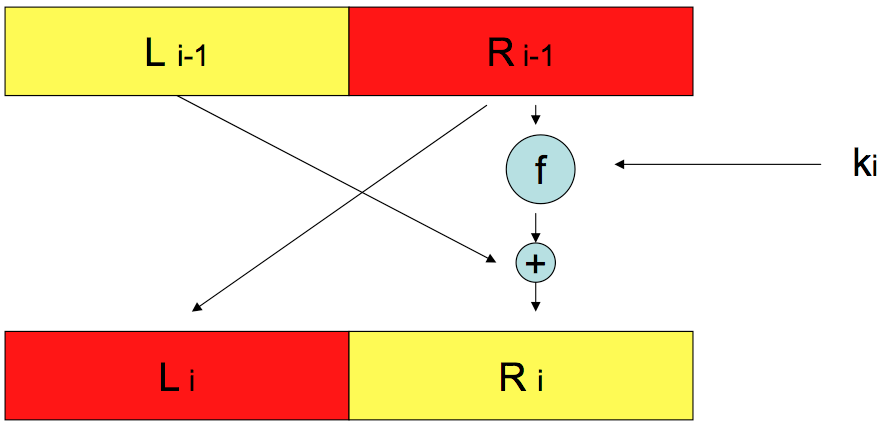
\includegraphics[scale=0.2]{horst-feistel.png}
\end{center}
\begin{align}
	L_1 & := R_0 \\
	R_1 & := f(R_0,k_1) \oplus L_0
\end{align}
\begin{align}
	L_0 & := f(L_1,k_1) \oplus R_1 \\
	R_0 & := L_1
\end{align}
\textbf{Die $f$-Funktion:} \\
\begin{center}
	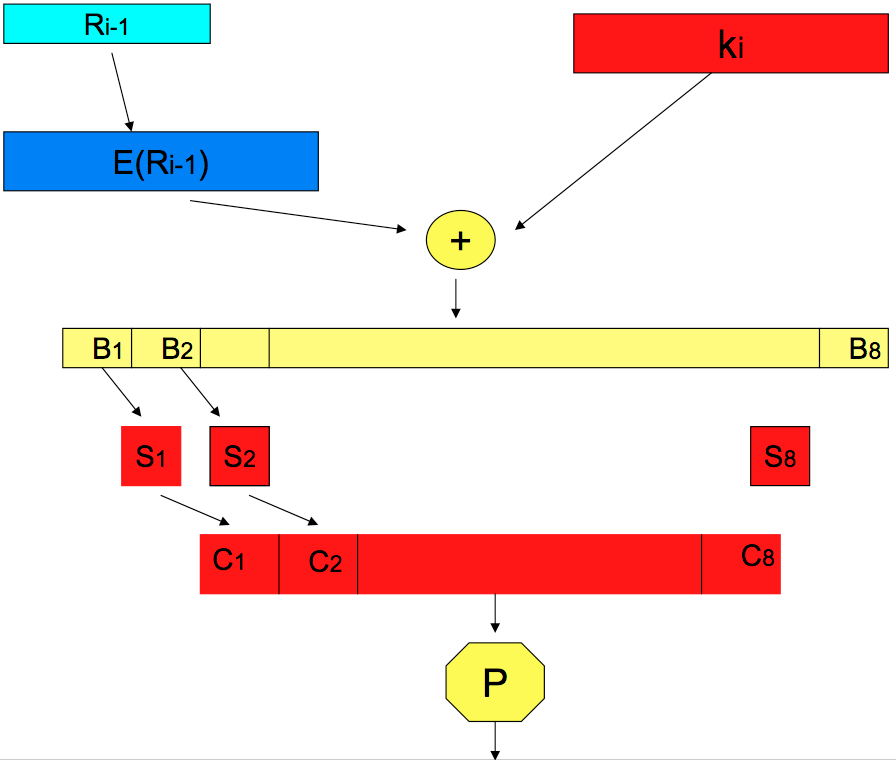
\includegraphics[scale=0.2]{funktion.png}
\end{center}

\subsection{Modi von Blocksipher}
Sei $\sum := \{0,1\}$ \\
P = C = $\sum^4$ \\
k = Permutationen von $\sum^4$ \\
k = $\pi$ = $(\frac{1 2 3 4}{2 1 3 4})$

\subsubsection*{Vor und Entschlüsselung}
Sei m=01001 $\in$ P (Klartext) \\
$e_k(m)=e_k(10101)=1010=C$

\subsubsection{ECB-Modul (Electornic Code Block)}
$m=\underbrace{1100}_{m_1}|\underbrace{0110}_{m_2} | \underbrace{1100}_{m_3} | 101*$ \\
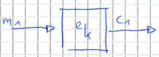
\includegraphics[scale=0.5]{ECB-modus.png}
\begin{description}
	\item[Bem. 1)] $m_1=m_3\Rightarrow c_1=c_3$
	\item[Bem. 2)] Vertauschen der Ciphertext-Blöcke wird nicht notwendigerweise erkannt.
\end{description}



\newpage
\section{Kryptosysteme}
\begin{description}
	\item[Kryptosystem:] (P, C, K, e, d)
	\item[P] Menge der {\color{blue}Klartexte}
	\item[C] Menge der {\color{red}Geheimtexte}
	\item[K] Menge der Schlüssel \\
		$e:K\times P \ra C$ \\
		$d:K\times C \ra P$ \\ \\
		$\forall k \varepsilon K$ $\forall p \varepsilon P: d( k, e (k,p))=p$ \\
		$\ra$ $\forall k \varepsilon K : e (k,-)$ ist {\color{blue}injektiv} \\
		$\ra$ $\forall k \varepsilon K : d (k,-)$ ist {\color{red}surjektiv} \\
\end{description}

\newpage
\section{Kryptoanalysis}
\subsection{Ciphertext-only attack}
\begin{description}
	\item[Gegeben] $c_i=e_k(p_i)$, i=1, ..., n
	\item[Gesucht] $p_i$, i= 1, ...,n oder k
\end{description}

\subsection{known-plaintext attack}
\begin{description}
	\item[Gegeben] ($p_i$, $c_i=e_k(p_i)$), i=1, ..., n
	\item[Gesucht] k
\end{description}

\subsection{chosen-plaintext attack}
\begin{description}
	\item[Gegeben] ($p_i$, $c_i=e_k(p_i)$), i=1, ..., n \\
		$p_i$ nach Wahl des Kryptoanalytikers
	\item[Gesucht] k
	\item[Verwendung] DIE Attacke gegen jedes Public-Key System
\end{description}

\subsection{chosen-ciphertext attack}
\begin{description}
	\item[Gegeben] ($p_i$, $p_i=d_k(c_i)$), i=1, ..., n \\
		$c_i$ nach Wahl des Kryptoanalytikers
	\item[Gesucht] k
\end{description}

% Inhalt Ende 
\end{document} 